% Section content template for individual Educative lessons
% This file contains the actual content for a specific section
% Generated from Educative API section content

% Section: Requirements for the Parking Lot Design
% Section ID: 4928023392681984
% Section Slug: requirements-for-the-parking-lot-design
% Generated: 2025-12-11T13:39:22.337084

In this lesson, we outline the functional and operational requirements for the parking lot system. Identifying and understanding requirements is essential to defining the system's scope and ensuring a robust, user-friendly design.
\\
We'll use the notational convention to identify each requirement with a unique label ``Rn,'' where ``R'' is short for requirement and ``n'' is a natural number.

\subsection{Requirements collection}\label{YNhB9OGSi3zqPM7pOjlmM}
\\
Let's define the requirements for the parking lot problem:

% \vspace{-1.0\baselineskip}
\noindent
\begin{minipage}[t]{0.48\textwidth}\vspace{0pt}
\begin{itemize}
\item
\textbf{R1:} The parking lot must support a total capacity of up to 40,000 vehicles.
\item
\textbf{R2:} The parking lot must support multiple types of parking spots:

\begin{itemize}
\tightlist
\item
Accessible (for individuals with disabilities)\\
\item
Compact
\item
Large
\item
Motorcycle
\end{itemize}
\item
\textbf{R3:} The parking lot should provide multiple entrance and exit points to support efficient traffic flow.
\end{itemize}
\end{minipage}
\hfill
\begin{minipage}[t]{0.48\textwidth}\vspace{0pt}
\centering
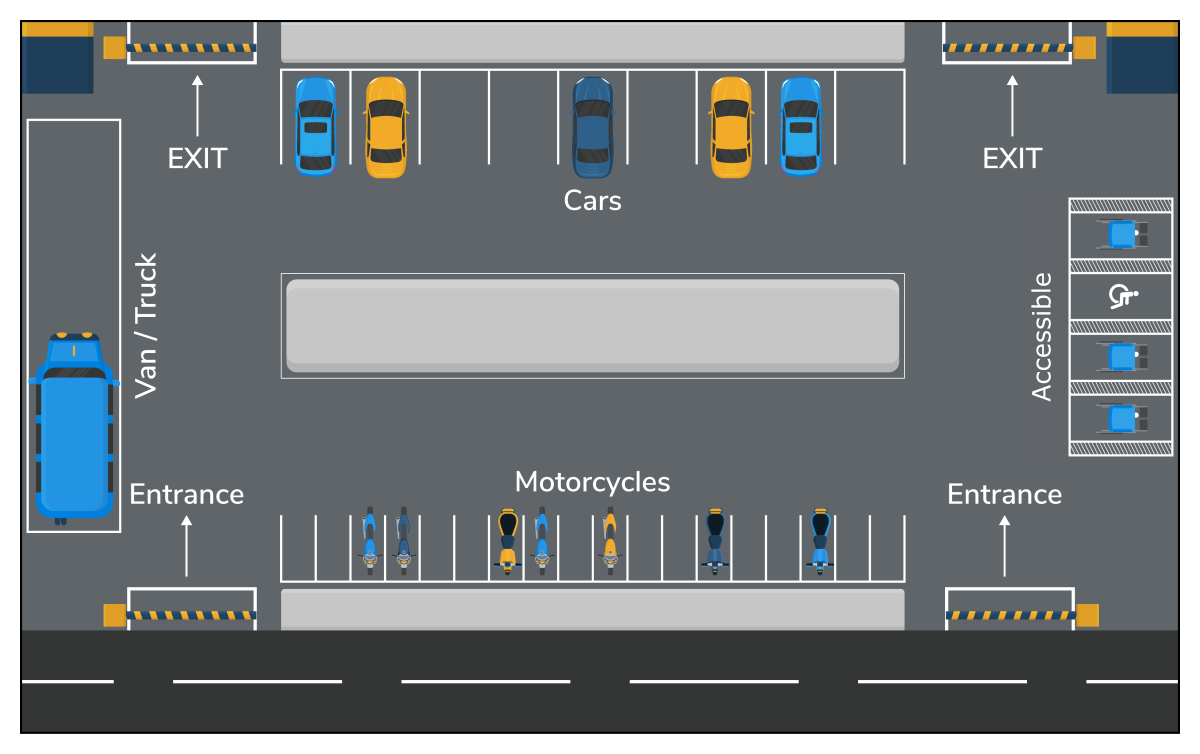
\includegraphics[width=0.5\textwidth]{Images/chapter_7/section_4928023392681984/6125700408803328.png}
\end{minipage}

% \vspace{-1.0\baselineskip}
\noindent
\begin{minipage}[t]{0.48\textwidth}\vspace{0pt}
\begin{itemize}
\tightlist
\item
\textbf{R4:} The system must support parking for four types of vehicles: cars, trucks, vans, and motorcycles.
\end{itemize}
\end{minipage}
\hfill
\begin{minipage}[t]{0.48\textwidth}\vspace{0pt}
\centering
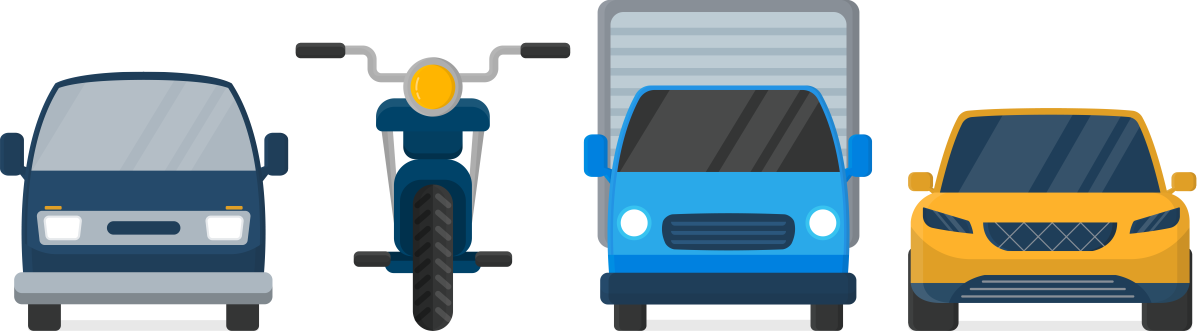
\includegraphics[width=0.5\textwidth]{Images/chapter_7/section_4928023392681984/5965407518457856.png}
\end{minipage}

% \vspace{-1.0\baselineskip}
\noindent
\begin{minipage}[t]{0.48\textwidth}\vspace{0pt}
\begin{itemize}
\item
\textbf{R5:} A display board at each entrance and on every floor should show the current number of available parking spots for each parking spot type.
\item
\textbf{R6:} The system must not allow more vehicles to enter once the parking lot reaches its maximum capacity.
\item
\textbf{R7:} When the parking lot is fully occupied, a clear message should be displayed at each entrance and on all display boards.
\end{itemize}
\end{minipage}
\hfill
\begin{minipage}[t]{0.48\textwidth}\vspace{0pt}
\centering
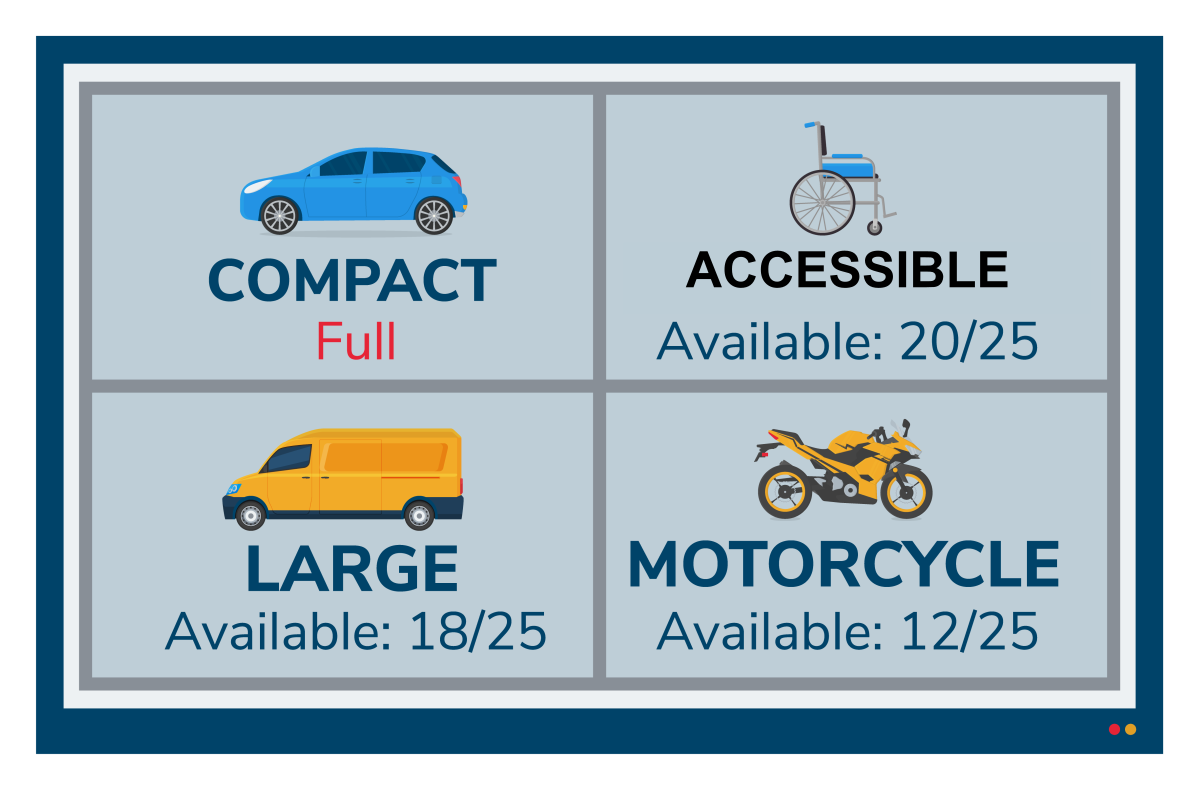
\includegraphics[width=0.5\textwidth]{Images/chapter_7/section_4928023392681984/6270981007867904.png}
\end{minipage}

% \vspace{-1.0\baselineskip}
\noindent
\begin{minipage}[t]{0.48\textwidth}\vspace{0pt}
\begin{itemize}
\item
\textbf{R8:} Customers must be issued a parking ticket at entry. The ticket will be used to track parking time and calculate payment at exit.
\item
\textbf{R9:} Customers should be able to pay for parking at the automated exit panel.
\item
\textbf{R10:} The parking lot system must support configurable pricing rates based on vehicle type and/or parking spot type and rates for different parking durations (e.g., first hour, subsequent hours).
\item
\textbf{R11:} Payments must be accepted via credit/debit card and cash at all payment points.
\end{itemize}
\end{minipage}
\hfill
\begin{minipage}[t]{0.48\textwidth}\vspace{0pt}
\centering
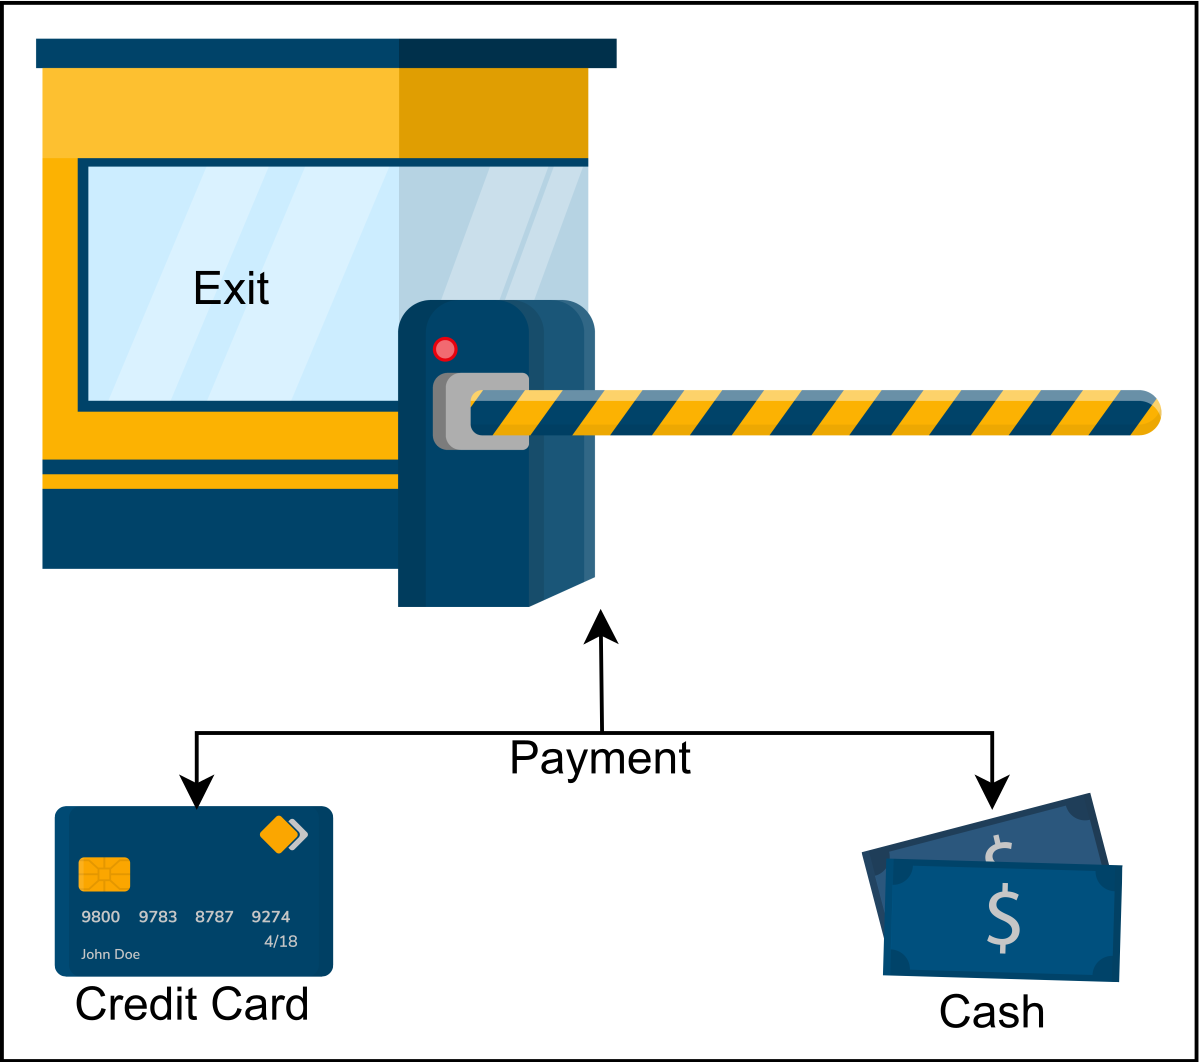
\includegraphics[width=0.5\textwidth]{Images/chapter_7/section_4928023392681984/6309111689117696.png}
\end{minipage}

We've identified the problem's requirements. Next, we will define different use cases for our parking lot system.

\subsection{}\label{262ynpMjkWFVZcetz0O5l}

% End of section content